% Options for packages loaded elsewhere
\PassOptionsToPackage{unicode}{hyperref}
\PassOptionsToPackage{hyphens}{url}
\PassOptionsToPackage{dvipsnames,svgnames,x11names}{xcolor}
%
\documentclass[
  11pt,
]{article}

\usepackage{amsmath,amssymb}
\usepackage{iftex}
\ifPDFTeX
  \usepackage[T1]{fontenc}
  \usepackage[utf8]{inputenc}
  \usepackage{textcomp} % provide euro and other symbols
\else % if luatex or xetex
  \usepackage{unicode-math}
  \defaultfontfeatures{Scale=MatchLowercase}
  \defaultfontfeatures[\rmfamily]{Ligatures=TeX,Scale=1}
\fi
\usepackage{lmodern}
\ifPDFTeX\else  
    % xetex/luatex font selection
\fi
% Use upquote if available, for straight quotes in verbatim environments
\IfFileExists{upquote.sty}{\usepackage{upquote}}{}
\IfFileExists{microtype.sty}{% use microtype if available
  \usepackage[]{microtype}
  \UseMicrotypeSet[protrusion]{basicmath} % disable protrusion for tt fonts
}{}
\makeatletter
\@ifundefined{KOMAClassName}{% if non-KOMA class
  \IfFileExists{parskip.sty}{%
    \usepackage{parskip}
  }{% else
    \setlength{\parindent}{0pt}
    \setlength{\parskip}{6pt plus 2pt minus 1pt}}
}{% if KOMA class
  \KOMAoptions{parskip=half}}
\makeatother
\usepackage{xcolor}
\usepackage[margin=1in]{geometry}
\setlength{\emergencystretch}{3em} % prevent overfull lines
\setcounter{secnumdepth}{5}
% Make \paragraph and \subparagraph free-standing
\makeatletter
\ifx\paragraph\undefined\else
  \let\oldparagraph\paragraph
  \renewcommand{\paragraph}{
    \@ifstar
      \xxxParagraphStar
      \xxxParagraphNoStar
  }
  \newcommand{\xxxParagraphStar}[1]{\oldparagraph*{#1}\mbox{}}
  \newcommand{\xxxParagraphNoStar}[1]{\oldparagraph{#1}\mbox{}}
\fi
\ifx\subparagraph\undefined\else
  \let\oldsubparagraph\subparagraph
  \renewcommand{\subparagraph}{
    \@ifstar
      \xxxSubParagraphStar
      \xxxSubParagraphNoStar
  }
  \newcommand{\xxxSubParagraphStar}[1]{\oldsubparagraph*{#1}\mbox{}}
  \newcommand{\xxxSubParagraphNoStar}[1]{\oldsubparagraph{#1}\mbox{}}
\fi
\makeatother


\providecommand{\tightlist}{%
  \setlength{\itemsep}{0pt}\setlength{\parskip}{0pt}}\usepackage{longtable,booktabs,array}
\usepackage{calc} % for calculating minipage widths
% Correct order of tables after \paragraph or \subparagraph
\usepackage{etoolbox}
\makeatletter
\patchcmd\longtable{\par}{\if@noskipsec\mbox{}\fi\par}{}{}
\makeatother
% Allow footnotes in longtable head/foot
\IfFileExists{footnotehyper.sty}{\usepackage{footnotehyper}}{\usepackage{footnote}}
\makesavenoteenv{longtable}
\usepackage{graphicx}
\makeatletter
\newsavebox\pandoc@box
\newcommand*\pandocbounded[1]{% scales image to fit in text height/width
  \sbox\pandoc@box{#1}%
  \Gscale@div\@tempa{\textheight}{\dimexpr\ht\pandoc@box+\dp\pandoc@box\relax}%
  \Gscale@div\@tempb{\linewidth}{\wd\pandoc@box}%
  \ifdim\@tempb\p@<\@tempa\p@\let\@tempa\@tempb\fi% select the smaller of both
  \ifdim\@tempa\p@<\p@\scalebox{\@tempa}{\usebox\pandoc@box}%
  \else\usebox{\pandoc@box}%
  \fi%
}
% Set default figure placement to htbp
\def\fps@figure{htbp}
\makeatother

\makeatletter
\@ifpackageloaded{caption}{}{\usepackage{caption}}
\AtBeginDocument{%
\ifdefined\contentsname
  \renewcommand*\contentsname{Table of contents}
\else
  \newcommand\contentsname{Table of contents}
\fi
\ifdefined\listfigurename
  \renewcommand*\listfigurename{List of Figures}
\else
  \newcommand\listfigurename{List of Figures}
\fi
\ifdefined\listtablename
  \renewcommand*\listtablename{List of Tables}
\else
  \newcommand\listtablename{List of Tables}
\fi
\ifdefined\figurename
  \renewcommand*\figurename{Figure}
\else
  \newcommand\figurename{Figure}
\fi
\ifdefined\tablename
  \renewcommand*\tablename{Table}
\else
  \newcommand\tablename{Table}
\fi
}
\@ifpackageloaded{float}{}{\usepackage{float}}
\floatstyle{ruled}
\@ifundefined{c@chapter}{\newfloat{codelisting}{h}{lop}}{\newfloat{codelisting}{h}{lop}[chapter]}
\floatname{codelisting}{Listing}
\newcommand*\listoflistings{\listof{codelisting}{List of Listings}}
\makeatother
\makeatletter
\makeatother
\makeatletter
\@ifpackageloaded{caption}{}{\usepackage{caption}}
\@ifpackageloaded{subcaption}{}{\usepackage{subcaption}}
\makeatother

\usepackage{bookmark}

\IfFileExists{xurl.sty}{\usepackage{xurl}}{} % add URL line breaks if available
\urlstyle{same} % disable monospaced font for URLs
\hypersetup{
  pdftitle={PSTAT 5A Practice Worksheet 2},
  pdfauthor={Student Name: \_\_\_\_\_\_\_\_\_\_\_\_\_\_\_\_\_\_\_\_\_\_\_\_},
  colorlinks=true,
  linkcolor={blue},
  filecolor={Maroon},
  citecolor={Blue},
  urlcolor={Blue},
  pdfcreator={LaTeX via pandoc}}


\title{PSTAT 5A Practice Worksheet 2}
\usepackage{etoolbox}
\makeatletter
\providecommand{\subtitle}[1]{% add subtitle to \maketitle
  \apptocmd{\@title}{\par {\large #1 \par}}{}{}
}
\makeatother
\subtitle{Descriptive Statistics}
\author{Student Name: \_\_\_\_\_\_\_\_\_\_\_\_\_\_\_\_\_\_\_\_\_\_\_\_}
\date{2025-07-02}

\begin{document}
\maketitle

\renewcommand*\contentsname{Table of contents}
{
\hypersetup{linkcolor=}
\setcounter{tocdepth}{3}
\tableofcontents
}

\section{Instructions and Overview}\label{instructions-and-overview}

\textbf{⏰ Time Allocation:} - \textbf{Section A (Warm-up):} 15 minutes

\begin{itemize}
\item
  \textbf{Section B (Intermediate):} 25 minutes
\item
  \textbf{Section C (Wrap-Up):} 10 minutes
\item
  \textbf{Total:} 50 minutes
\end{itemize}

\textbf{📝 Important Instructions:}

\begin{itemize}
\item
  Use the formulas provided for guidance
\item
  Round final answers to 4 decimal places unless otherwise specified
\item
  Identify your approach before calculating
\item
  Use calculator as needed
\end{itemize}

\textbf{📚 Key Formulas Reference:}

\textbf{DESCRIPTIVE STATISTICS:}

\textbf{1. Mean Formulas:}

\begin{itemize}
\item
  Sample Mean: \(\bar x = \frac{\sum x_i}{n}\)
\item
  Population Mean: \(\mu = \frac{\sum x_i}{N}\)
\end{itemize}

\textbf{2. Variance Formulas:}

\begin{itemize}
\item
  Population Variance:
  \(\sigma^2 = \frac{\sum_{i=1}^{N} (x_i - \mu)^2}{N}\)
\item
  Sample Variance:
  \(s^2 = \frac{\sum_{i=1}^{n} (x_i - \bar{x})^2}{n-1}\)
\end{itemize}

\textbf{3. Standard Deviations Formulas:}

\begin{itemize}
\item
  Sample Standard Deviation:
  \(s = \sqrt \frac{\sum (x_i - \bar x)^2}{(n-1)}\)
\item
  Population Standard Deviation:
  \(\sigma = \sqrt \frac{\sum (x_i - \mu)^2}{N}\)
\end{itemize}

\textbf{MEASURES OF POSITION:}

\begin{itemize}
\item
  Percentile: Value below which a certain percentage of data falls
\item
  Quartiles: Q1 (25th percentile), Q2 = Median (50th percentile), Q3
  (75th percentile)
\item
  Interquartile Range (IQR): Q3 - Q1
\item
  Range: Maximum - Minimum
\end{itemize}

\textbf{DISTRIBUTION SHAPES:}

\begin{itemize}
\item
  Symmetric: Mean ≈ Median
\item
  Right-skewed: Mean \textgreater{} Median (tail extends to the right)
\item
  Left-skewed: Mean \textless{} Median (tail extends to the left)
\item
  Outliers affect the mean more than the median
\end{itemize}

\section{Section A: Basic Descriptive
Statistics}\label{section-a-basic-descriptive-statistics}

\emph{⏱️ Estimated time: 15 minutes}

\textbf{Problem A1: Mean and Standard Deviation}

In a class of 25 students, 24 of them took an exam in class and 1
student took a make-up exam the following day. The professor graded the
first batch of 24 exams and found an average score of 74 points with a
standard deviation of 8.9 points. The student who took the make-up the
following day scored 64 points on the exam.

\begin{enumerate}
\def\labelenumi{(\alph{enumi})}
\tightlist
\item
  Does the new student's score increase or decrease the average score?
\item
  What is the new average?
\item
  Does the new student's score increase or decrease the standard
  deviation of the scores?
\end{enumerate}

\textbf{Answer:}

\textbf{Problem A2: Distribution Shape Analysis}

Students in an AP Statistics class were asked how many hours of
television they watch per week (including online streaming). This sample
yielded an average of 4.71 hours, with a standard deviation of 4.18
hours. Is the distribution of number of hours students watch television
weekly symmetric? If not, what shape would you expect this distribution
to have? Explain your reasoning

\textbf{Answer:}

\section{Section B: Data Interpretation and Graphical
Analysis}\label{section-b-data-interpretation-and-graphical-analysis}

\emph{⏱️ Estimated time: 25 minutes}

\textbf{Problem B1: Interpreting Histograms}

The infant mortality rate is defined as the number of infant deaths per
1,000 live births. This rate is often used as an indicator of the level
of health in a country. The relative frequency histogram below shows the
distribution of estimated infant death rates for 224 countries for which
such data were available in 2014.

\begin{enumerate}
\def\labelenumi{(\alph{enumi})}
\tightlist
\item
  Estimate Q1, the median, and Q3 from the histogram.
\item
  Would you expect the mean of this data set to be smaller or larger
  than the median? Explain your reasoning.
\end{enumerate}

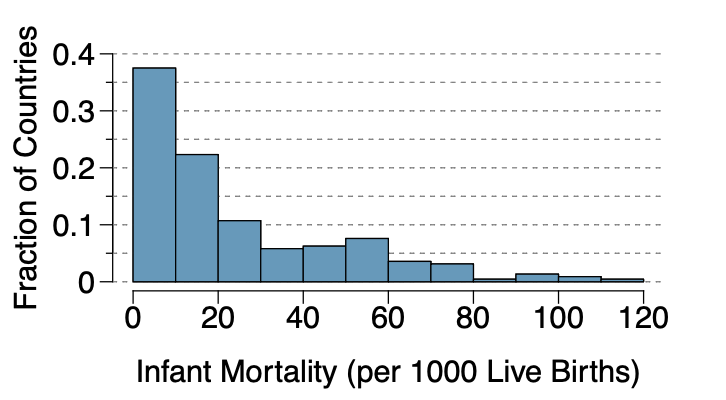
\includegraphics[width=1\linewidth,height=\textheight,keepaspectratio]{../../files/worksheets/img/infant_mortality.png}

\textbf{Answer:}

\textbf{Problem B2: Comparing Distributions}

Use the plots in the Figure below to compare the incomes for counties
across the two groups. What do you notice about the approximate center
of each group? What do you notice about the variability between groups?
Is the shape relatively consistent between groups? How many prominent
modes are there for each group?

\pandocbounded{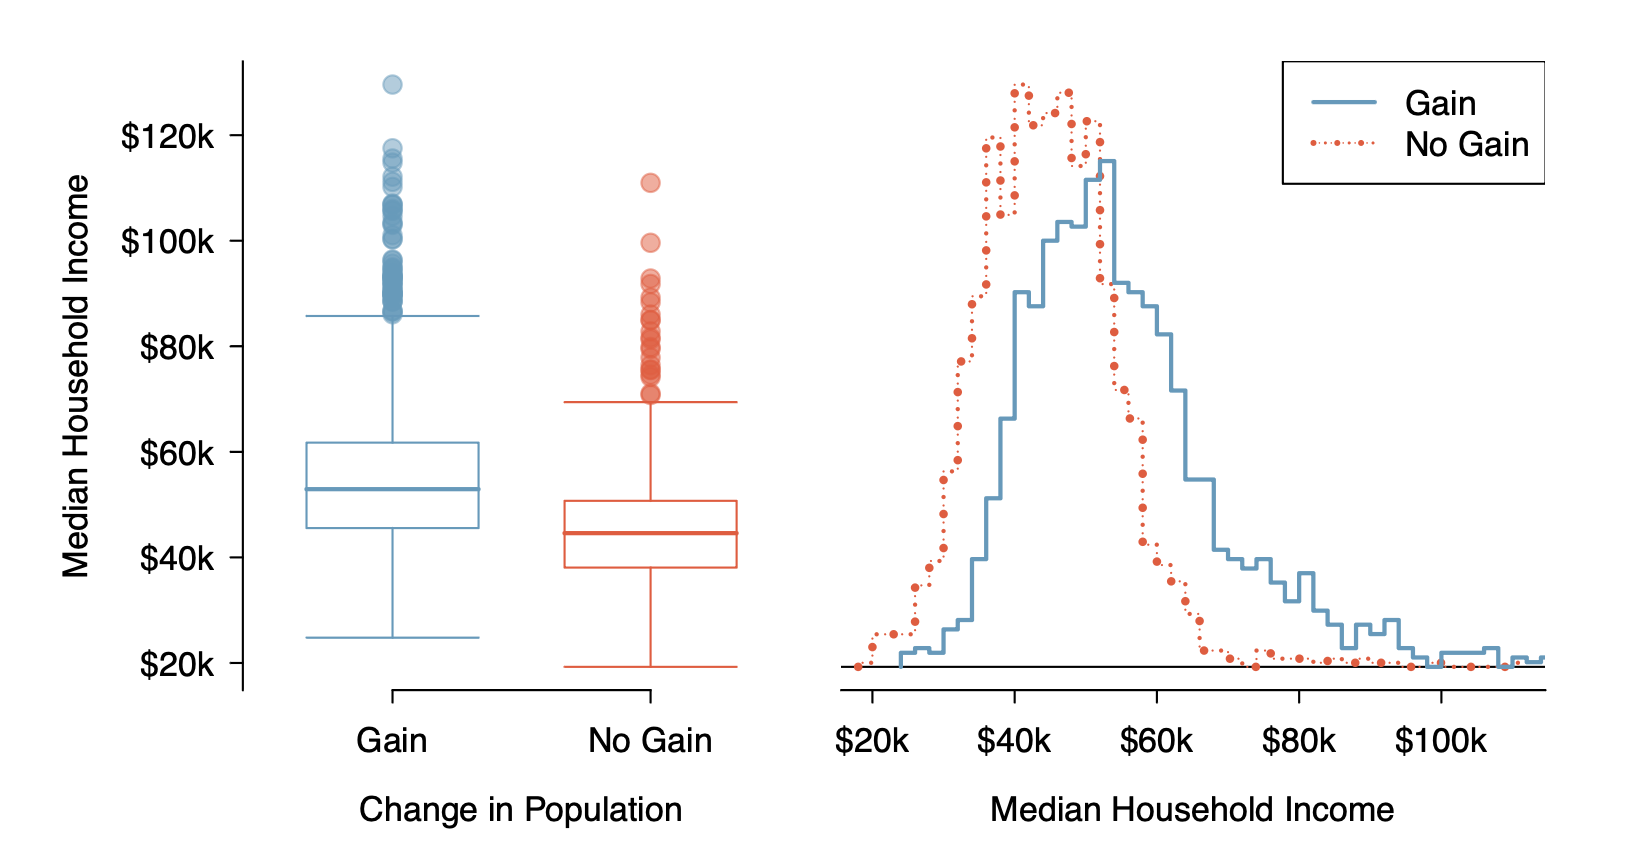
\includegraphics[keepaspectratio]{../../files/worksheets/img/plots.png}}

\textbf{Answer:}

\section{Section C : Variance Calculations
Practice}\label{section-c-variance-calculations-practice}

\emph{⏱️ Estimated time: 10 minutes}

\subsection{Understanding Variance: Population vs
Sample}\label{understanding-variance-population-vs-sample}

\textbf{🎯 Key Variance Concepts:}

\textbf{Population Variance} (when you have ALL data):
\[\sigma^2 = \frac{\sum_{i=1}^{N} (x_i - \mu)^2}{N}\]

\textbf{Sample Variance} (when you have a sample):
\[s^2 = \frac{\sum_{i=1}^{n} (x_i - \bar{x})^2}{n-1}\]

\textbf{Why (n-1)?} Using the sample mean to estimate deviations ``uses
up'' one degree of freedom.

\textbf{Problem C1: Basic Variance Calculations}

The following data represents the number of customer complaints per day
for a small business over 8 days:

\textbf{Data:} 3, 7, 2, 8, 5, 6, 4, 9

\textbf{Part (a) :} Calculate the sample mean \(\bar{x}\).

\textbf{Part (b) :} Calculate the sample variance \(s^2\) using the
formula with \((n-1)\) in the denominator.

\textbf{Part (c) :} Calculate the sample standard deviation \(s\).

\textbf{Part (d) :} If this were treated as a complete population, what
would the population variance \(\sigma^2\) be?

\textbf{Part (e) :} Explain why we divide by \((n-1)\) for sample
variance instead of \(n\).

\textbf{Answer:}

\textbf{Problem C2: Comparing Variability}

Consider two data sets:

\begin{itemize}
\item
  Set A: 10, 12, 14, 16, 18
\item
  Set B: 5, 10, 14, 18, 23
\end{itemize}

\begin{enumerate}
\def\labelenumi{(\alph{enumi})}
\tightlist
\item
  Calculate the mean for each set.
\item
  Calculate the sample variance for each set.
\item
  Which set has greater variability?
\item
  Calculate the coefficient of variation \((CV = s/x̄)\) for each set.
  Which has greater relative variability?
\end{enumerate}

\textbf{Answer:}




\end{document}
